\documentclass[protocolo.tex]{subfiles}
\usepackage{graphicx}
\begin{document}

\section{Resultados}
Todo proyecto realizado es operacional y se encuentra actualmente en funcionamiento. La retroalimentación positiva recibida por parte de los superiores confirma la calidad del trabajo como Ingeniero en Software. Se ha manejado con éxito la calidad, gestión, diseño y desarrollo en cada uno de los proyectos en los que se ha trabajado, dejando una huella positiva en las empresas donde se ha colaborado.\vspace{4mm}

Como próximo ingeniero en software, se reconoce que aún queda mucho por aportar y crecer. Si bien sus errores han sido pocos, se esta consciente de que, como principiante, se cometieron algunos.  Sin embargo, se considera parte del proceso de aprendizaje en este campo laboral y nunca se permitió que afectaran al desarrollo de los proyectos al entorno laboral.\vspace{4mm}

Una aportación principal dentro de la experiencia adquirida ha sido la inteligencia emocional, la cual le ha permitido relacionarse mejor con sus compañeros de trabajo, superiores e incluso con personas ajenas a la empresa, como clientes o personal en capacitación. Se reconoce la importancia de manejar las diferentes posibilidades que puedan surgir dentro de un gran proyecto de desarrollo de software.

\subsection{Resultados del proyecto \textit{DataFire}}

El proyecto \textit{DataFire} consistió en el desarrollo de un sistema financiero empresarial para la gestión de costos, pago de nóminas y presupuestos de proyectos. Este sistema se implementó con el objetivo de optimizar la administración del dinero de la compañía y mejorar el control sobre las actividades dentro de los proyectos.\vspace{4mm}

Como resultados de la implementación de \textit{DataFire}, se logró:

\begin{itemize}
\item Reducir los gastos de la empresa en un 50\% gracias a la automatización de procesos y la optimización de recursos.
\item Mejorar la detección del rendimiento de los empleados, lo que permitió identificar áreas de oportunidad y tomar decisiones más informadas sobre la asignación de recursos humanos.
\end{itemize}

El proyecto \textit{DataFire} le permitió adquirir experiencia en el desarrollo de sistemas financieros empresariales y fortalecer las habilidades en el análisis de datos, la gestión de bases de datos y la programación en \textit{Flutter} y \textit{NodeJs}.

\subsection{Diagrama de flujo \textit{DataFire} }
\textbf{Funcionamiento:}
\begin{enumerate}
    \item \textbf{Inicio y Selección de Módulo:}  
    El diagrama inicia con el usuario que se autentica y luego selecciona el módulo que desea gestionar.
    \item \textbf{Decisiones por Módulo:} 
    \item Se utilizan nodos de decisión para determinar cuál módulo se va a gestionar:
        \begin{itemize}
            \item \textbf{Gestión Financiera:}  Permite administrar transacciones y generar reportes..
            \item \textbf{Gestión de Proyectos:}  Incluye la administración de proyectos, presupuesto, asignación de recursos y pagos o abonos.
            \item \textbf{Gestión de Personas:}  Cubre el alta de personas, asignación a proyectos, pago de nómina y gestión de usuarios.
            \item \textbf{Visualización:} Ofrece opciones para ver dashboards, gráficas y reportes de nóminas.
        \end{itemize}
    \item \textbf{Selección Reiterada y Finalización:} 
    Después de gestionar un módulo, el diagrama permite volver a seleccionar otro módulo, hasta finalizar la sesión.
\end{enumerate}

A continuación en la Figura 1 se muestra el diagrama de flujo del sistema \textit{DataFire}:\vspace{2mm}

\begin{center}
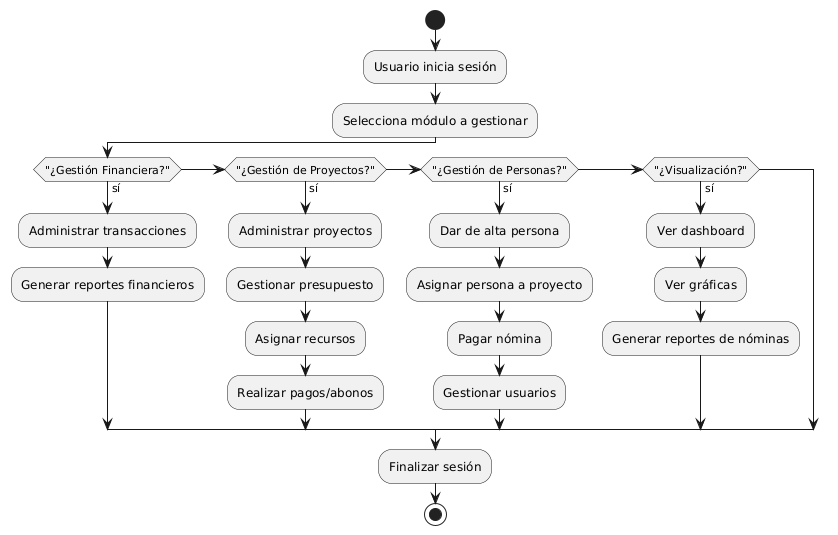
\includegraphics[width=0.75\textwidth]{Imagenes/datafireF2.png}
\end{center}
\begin{figure}[h]  % 'htbp' indica las posiciones preferidas: here, top, bottom, page
    \centering
    \caption{Diagrama de flujo DataFire.}
    \label{fig:mi-figura}
\end{figure}



\subsection{Resultados del proyecto \textit{VehicleTracking}}

El proyecto  \textit{VehicleTracking} se centró en el desarrollo de un sistema de conteo de vehículos con inteligencia artificial (IA) para el aforo vehicular.  Este sistema, aún en versión de pruebas, se implementó con el objetivo de automatizar el conteo de vehículos y reducir la necesidad de intervención humana en esta tarea.\vspace{4mm}

Como resultado de las pruebas de \textit{VehicleTracking}, se observó:

\begin{itemize}
\item Un aumento del 30\% en la eficiencia del conteo vehicular,  logrado gracias a la automatización del proceso mediante el uso de IA.
\end{itemize}

El proyecto \textit{VehicleTracking} le permitió adquirir experiencia en el desarrollo de sistemas de visión artificial y aprendizaje automático, así como en el procesamiento de imágenes y la programación en  \textit{Python},  \textit{YOLO} y  \textit{Ultralytics}.  Además, le brindó la oportunidad de trabajar con tecnologías de vanguardia y contribuir a la automatización de procesos en el ámbito del aforo vehicular.

\subsection{Diagrama de flujo \textit{VehicleTracking}} 
\textbf{Funcionamiento:}
\begin{enumerate}
    \item \textbf{Inicio:}  
    El usuario abre el sistema.
    \item \textbf{Selección de archivo:}  
    El usuario elige el video que desea procesar.
    \item \textbf{Reproducción:}  
    Puede (opcionalmente) iniciar la reproducción y controlarla (pausar, avanzar, retroceder).
    \item \textbf{Análisis con IA:}
    Se realiza el análisis del video para la detección de vehículos.
    \item \textbf{Reporte:}
    Se genera el reporte de conteo de vehículos.
    \item \textbf{Fin:}      
    El usuario finaliza la sesión o cierra el sistema.
\end{enumerate}

A continuación en la Figura 2 se muestra el diagrama de flujo del sistema \textit{VehicleTracking}:\vspace{4mm}

\begin{center}
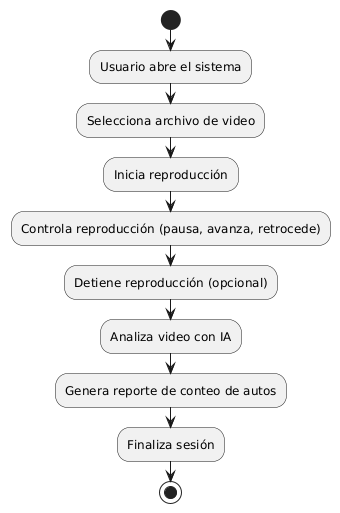
\includegraphics[scale=0.6]{Imagenes/pdf/VehicleTkF.png}
\end{center}
\begin{figure}[h]  % 'htbp' indica las posiciones preferidas: here, top, bottom, page
    \centering
    \caption{Diagrama de flujo VehicleTracking.}
    \label{fig:mi-figura2}
\end{figure}

\subsection{Resultados del proyecto CRM}

El proyecto CRM consistió en el desarrollo de un oyente basado en conexiones TCP/IP, que procesara datos en hexadecimal que contiene información telemétrica y geoespacial para posteriormente ingresarlos en la nube y poder visualizar los datos de manera constante y eficiente. \vspace{4mm}

Como resultado del desarrollo del CRM, se logró:

\begin{itemize}
    \item Una eficiencia del 80\% al cambiar de lenguaje de programación a python porque c++ no contenia la suficiente documentacion y robustez, esto ayudó a que el sistema fuera más rápido, entendible y escalable.
\end{itemize}

Estos resultados ayudaron a que la empresa ofreciera un mejor servicio de \textit{tracking} para las empresas que gozaban de estos beneficios al contar con Calamp integrado en sus unidades. \vspace{4mm}

El sistema CRM le permitió adquirir conocimientos para realizar un oyente para posteriormente procesar y manejar datos en hexadecimal además de fortalecer las habilidades de Héctor Hugo en lenguaje \textit{Python} y crecer en el ámbito de las conexiones TCP/IP.

\subsection{Caso de uso \textit{CRM}} 
\textbf{Funcionamiento:}
\begin{enumerate}
    \item \textbf{Receptor de Datos Hexadecimales:}  
    Este componente recibe datos geoespaciales en formato hexadecimal y decodifica a un formato más manejable
    \item \textbf{Transformador a Datos Geográficos:}  
    Toma la información decodificada por el receptor y la convierte en coordenadas geográficas y una vez obtenida las envía al visualizador.
    \item \textbf{Visualizador de Geolocalización:}  
    Recibe los datos geográficos y los muestra de forma visual, sobre un mapa.
\end{enumerate}
a continuación en la Figura 3 se muestra el diagrama de flujo del sistema CRM:\vspace{4mm}
\begin{center}
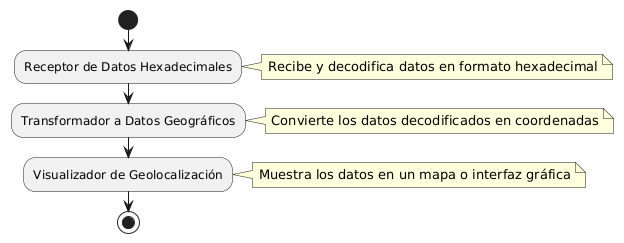
\includegraphics[scale=0.6]{Imagenes/pdf/crmF.png}
\end{center}
\begin{figure}[h]  % 'htbp' indica las posiciones preferidas: here, top, bottom, page
    \centering
    \caption{Diagrama de flujo CRM.}
    \label{fig:mi-figura3}
\end{figure}

\subsection{Resultados del proyecto \textit{FollowMe}}

El proyecto \textit{FollowMe} consistió en el desarrollo de un sistema para visualizar tráilers con cargas importantes mediante \textit{GoogleMaps}.  Se utilizó un dispositivo llamado Calamp que emitía señales en hexadecimal, para lo cual se desarrolló un oyente llamado CRM que capturaba la información y  actualizaba la base de datos con la ubicación en tiempo real.  Además, se implementó una vista para visualizar la ubicación y la telemetría del tráiler, con el fin de capturar datos y tomar medidas en tiempo real en caso de cualquier circunstancia.\vspace{4mm}

Como resultado de la implementación de \textit{Followme}, se logró:

\begin{itemize}
\item Una mejora del 80\% en la eficiencia del seguimiento de tráileres, ya que la información se  presentó  de forma más accesible y organizada para el personal encargado.
\end{itemize}

El proyecto \textit{Followme} permitió adquirir experiencia en el desarrollo de sistemas de rastreo en tiempo real y la integración con dispositivos de hardware. También brindó la oportunidad de aplicar las habilidades en la gestión de bases de datos y el desarrollo de interfaces de usuario.

\subsection{Diagrama de flujo \textit{FollowMe}} 
\textbf{Funcionamiento:}
\begin{enumerate}
    \item \textbf{Inicio:}  
    El usuario abre o inicia la aplicación \textit{FollowMe}.
    \item \textbf{Ingreso de Datos:}  
    El usuario ingresa el código del contenedor que desea consultar.
    \item \textbf{Ver Ubicación en Mapa:}  
    \begin{itemize}
        \item El usuario ve la ubicación, el sistema muestra un mapa con la posición del contenedor.
       
    \end{itemize}
    \item \textbf{Ver Cálculo de Distancia:} 
    \begin{itemize}
        \item El usuario desea conocer la distancia o el estado de proximidad, el sistema realiza el cálculo y lo muestra.
        
    \end{itemize}
    \item \textbf{Ver Información del Contenedor:} 
    Ver la información del contenedor, el sistema presenta:
    \item \begin{itemize}
        \item Información general (detalles, estado, etc.).
        \item Nivel de combustible.
        \item Velocidad.
        \item Temperatura del contenedor.
    \end{itemize}
    \item \textbf{Fin:} 
    El proceso termina cuando el usuario decide no ver más información o cierra la aplicación.
\end{enumerate}
A continuación en la Figura 4 se muestra el diagrama de flujo del sistema \textit{FollowMe}:\vspace{4mm}
\begin{center}
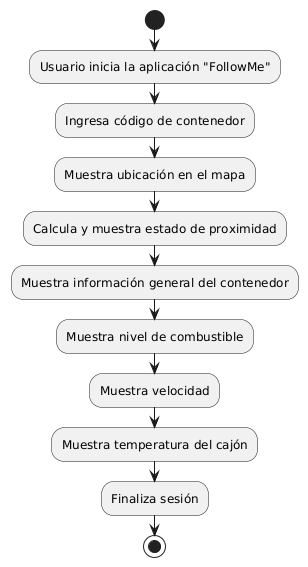
\includegraphics[scale=0.6]{Imagenes/Pdf/followmeF.png}
\end{center}
\begin{figure}[h]  % 'htbp' indica las posiciones preferidas: here, top, bottom, page
    \centering
    \caption{Diagrama de flujo FollowMe.}
    \label{fig:mi-figura4}
\end{figure}
\subsection{Resultados del proyecto AdCom}

El proyecto AdCom se enfocó en el desarrollo de un sistema de administración de fraccionamientos con el objetivo de  mejorar la comunicación entre la administración y los residentes,  facilitar el acceso a la información y agilizar los procesos administrativos.  A través de este sistema, los residentes pueden  familiarizarse con su residencia,  disfrutar de sus recursos,  consultar sus deudas y realizar pagos de forma online.\vspace{4mm}

Como resultados de la implementación de Adcom, se logró:

\begin{itemize}
\item Una reducción del 90\% en las llamadas al personal de asistencia,  gracias a la disponibilidad de información y la  facilidad  de  uso  del  sistema.
\item Una mejora del 50\% en los reportes de incidentes dentro del fraccionamiento,  al  proporcionar  un  canal  de  comunicación  más  eficiente  y  accesible  para  los  residentes.
\item Una reducción del 100\% en el tiempo dedicado a la gestión de pagos,  al  implementar  un  sistema  de  pagos  vía  móvil.
\end{itemize}

Estos resultados contribuyeron a que la empresa  optimizara la administración de su personal, liberando tiempo para dedicarlo a otras tareas que requerían  mayor  atención.\vspace{4mm}

El proyecto Adcom permitió adquirir experiencia en el desarrollo de sistemas web para la gestión de comunidades,  la integración de pasarelas de pago y la  implementación  de  sistemas  de  notificación.  Además,  fortaleció  las  habilidades  en  el  diseño  de  interfaces  de  usuario  intuitivas  y  la  gestión  de  proyectos  con  enfoque  en  la  experiencia  del  usuario.

\subsection{Diagrama de flujo \textit{AdCom}} 

\textbf{Funcionamiento:}

\begin{enumerate}
    \item \textbf{Inicio de Sesión:}  
    El actor (Usuario o Administrador) se autentica en la aplicación.
    \item \textbf{Áreas:} 
    \begin{itemize}
        \item \textbf{Gestionar Pagos:}  Quien lo elige (usuario o admin) puede realizar las tareas correspondientes (pagar renta, ver adeudos, generar reportes, etc.).
        \item \textbf{Gestionar Reportes:}  Se generan o consultan reportes, y el administrador puede responder o actualizar reportes y mensajes.
        \item \textbf{Gestionar Amenidades:}  Se pueden reservar, cancelar o ver disponibilidad de amenidades. El administrador, además, gestiona la configuración general de estas.
    \end{itemize} 
    
    \item \textbf{Fin:}  
    Cuando el actor ya no necesita hacer más acciones, sale de la aplicación.

\end{enumerate}
A continuación en la Figura 5 se muestra el diagrama de flujo del sistema AdCom:\vspace{4mm}
\begin{center}
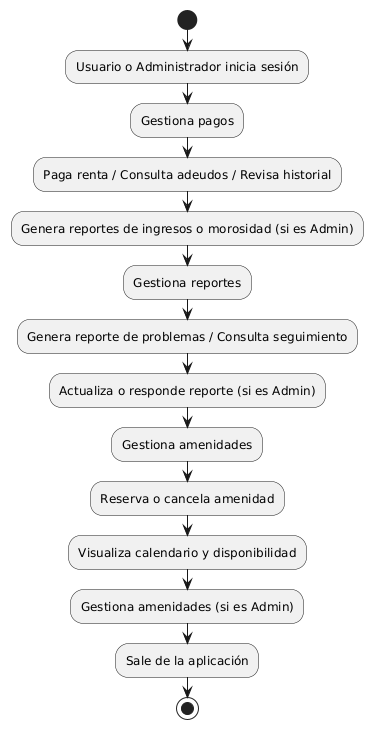
\includegraphics[scale=0.5]{Imagenes/Pdf/AdcomF.png}
\end{center}
\begin{figure}[h]  % 'htbp' indica las posiciones preferidas: here, top, bottom, page
    \centering
    \caption{Diagrama de flujo AdCom.}
    \label{fig:mi-figura5}
\end{figure}

\subsection{Resultados del proyecto Zae}

El proyecto Zae consistió en el desarrollo e implementación de un sistema ERP para la gestión integral de las empresas del Grupo Tomza. Este sistema se diseñó para administrar las ventas, empleados, facturas, encargos, llamadas y reportes de las plantas en los diferentes estados de México.\vspace{4mm}

Como resultado de la implementación de Zae, se logró:

\begin{itemize}
\item Una mejora del 90\% en la visualización de datos,  facilitando el acceso a la información relevante para la toma de decisiones.
\item Un aumento del 70\% en la eficiencia de la generación de reportes,  agilizando los procesos administrativos y operativos.
\item Un incremento del 80\%o en las ventas de gas,  gracias a la mejora en la calidad, rendimiento y usabilidad del sistema.
\end{itemize}

Zae se convirtió en el sistema clave de la empresa,  permitiendo una mejor gestión de las ventas y una visión más completa del estado general de la compañía.\vspace{4mm}

El proyecto Zae le permitió adquirir experiencia en el desarrollo e implementación de sistemas ERP,  la integración de diferentes módulos y la gestión de bases de datos a gran escala. Además, fortaleció las habilidades en el análisis de requerimientos, el diseño de soluciones  y  el  trabajo  en  equipo  con  diferentes  áreas  de  la  empresa.\vspace{4mm}

\subsection{Diagrama de flujo \textit{Zae}} 
\textbf{Funcionamiento:}
\begin{enumerate}
    \item \textbf{Inicio: }  
    El usuario inicia sesión en el sistema.
    \item \textbf{Administrar Ventas y Facturación:}  
    El usuario puede (o no) realizar la venta y facturación en ese momento.
    \item \textbf{Administrar Gas:}  
    Si corresponde, gestiona inventario de gas y registra cuentas por pagar a los proveedores.
    \item \textbf{Administrar Empleados:} 
    Opcionalmente, el usuario puede crear, modificar o dar de baja empleados.
    \item \textbf{Apertura/Cierre de Caja:} 
    Para controlar el flujo de efectivo, se realiza la apertura y/o cierre de caja cuando sea necesario.
    \item \textbf{Fin:}
    El proceso concluye cuando el usuario no tiene más acciones que realizar.  
\end{enumerate}

A continuación en la Figura 6 se muestra el diagrama de flujo del sistema Zae:\vspace{4mm}


\begin{center}
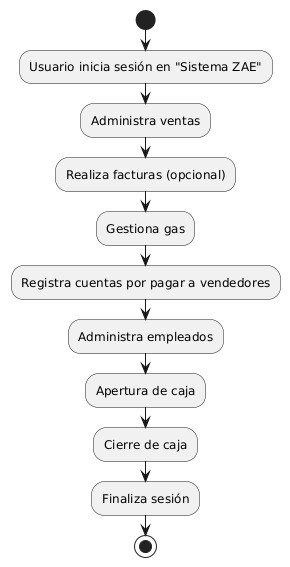
\includegraphics[scale=0.6]{Imagenes/Pdf/zaeF.png}
\end{center}
\begin{figure}[h]  % 'htbp' indica las posiciones preferidas: here, top, bottom, page
    \centering
    \caption{Diagrama de flujo Zae.}
    \label{fig:mi-figura6}
\end{figure}
\subsection{Resultados del proyecto Zae Ejecutivo}

El proyecto Zae Ejecutivo se enfocó en el desarrollo de un sistema web que globaliza los datos del sistema Zae y los presenta de forma visual con gráficos  y  datos  concretos.  Este sistema se diseñó para  facilitar  la  comprensión  de  métricas  clave  como  las  ventas,  el  rendimiento  de  presupuestos  y  el  rendimiento  de  las  plantas,  y  permitir  la  creación  de  reportes  globales.  Zae  Ejecutivo  se  orientó  a  gerentes  y  altos  ejecutivos  de  la  compañía.\vspace{4mm}

Como resultado de la implementación de Zae Ejecutivo, se logró:

\begin{itemize}
\item Una mejora del 85\%  en la visualización y el entendimiento de los datos por parte de los encargados de nivel mayor,  facilitando la toma de decisiones estratégicas.
\item Un aumento del 70\% en la usabilidad y en el rendimiento del sistema, garantizando así la disponibilidad y estabilidad de la información que ofrece el sistema.
\end{itemize}

Zae Ejecutivo logró que los ejecutivos de la empresa administraran mejor sus recursos y  planearan mejor  sus  próximos  movimientos  en  base a información confiable  y  actualizada.\vspace{4mm}

El proyecto Zae Ejecutivo le permitió adquirir experiencia en el desarrollo de sistemas de  \textit{business intelligence}, la visualización de datos y la creación de  \textit{Dashboards}  interactivos. Además, fortaleció las habilidades en  el  diseño  de interfaces  de  usuario  para  altos  ejecutivos y la presentación de información de forma clara  y concisa.

\subsection{Diagrama de flujo \textit{Zae Ejecutivo}}
\textbf{Funcionamiento:}
\begin{enumerate}
    \item \textbf{Inicio de sesión: }  
    \begin{itemize}
        \item El usuario abre la aplicación “Zae Ejecutivo” e inicia sesión.
        \item Este paso inicial establece el punto de partida para realizar cualquier acción dentro del sistema.
        
    \end{itemize}
    \item \textbf{Ver reportes financieros:}  
    \begin{itemize}
        \item Consultar reportes financieros, entra a esa sección.
        \item Dentro de esta sección, el sistema muestra ganancias y pérdidas.
        
        
    \end{itemize}
    \item \textbf{Ver estadísticas en dashboard:}  
    \begin{itemize}
        \item Ver las estadísticas generales (en un dashboard).
        \item Se muestran métricas globales o indicadores claves del negocio (ventas totales, comparativas, etc.).
        
        
    \end{itemize}
    \item \textbf{Consultar ventas:} 
    \begin{itemize}
        \item Consultar las ventas en distintos rangos de tiempo: día, semana, mes o año.
        \item Esta parte puede ayudar a entender la evolución de las ventas y patrones de consumo.
        
        
    \end{itemize}
    \item \textbf{Consultar sucursales:} 
    \begin{itemize}
        \item En caso de tener múltiples sucursales, el sistema permite ver cuáles tienen mejores o peores ventas, así como un reporte de otras sucursales.
        \item El usuario revisa esta información si la necesita.
        
        
    \end{itemize}
    \item \textbf{Administrar empleados:}
    El usuario puede:
    \begin{itemize}
        \item Dar de alta nuevos empleados.
        \item Dar de baja empleados que ya no laboran.
        \item Asignar roles (ej. cajero, gerente, etc.).
        \item Ver el mejor vendedor de la zona (por ejemplo, basado en metas de venta).
        

    \end{itemize}
    \item \textbf{Gestionar presupuestos:} 
   \begin{itemize}
        \item El sistema ofrece la generación de permisos de presupuestos (probablemente para autorizar compras o gastos).
        \item Se lleva a cabo solo si el usuario tiene la necesidad de hacerlo.

    \end{itemize}
    \item \textbf{Consultar conciliaciones:}
    \begin{itemize}
        \item El usuario puede ver la conciliación de cuentas o movimientos financieros para asegurar que coincidan con registros bancarios o contables.
        \item Se hace únicamente cuando es pertinente.

    \end{itemize}
    \item \textbf{Fin:}  
    \begin{itemize}
        \item El flujo termina cuando el usuario no requiere más acciones o cierra la aplicación.
    \end{itemize}
\end{enumerate}

A continuación en la Figura 7 se muestra el diagrama de flujo del sistema Zae Ejecutivo:\vspace{4mm}



\begin{center}
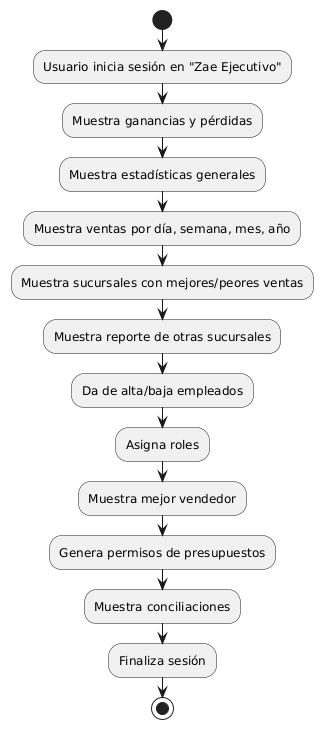
\includegraphics[scale=0.6]{Imagenes/Pdf/zaeejecutivoF.png}
\end{center}
\begin{figure}[h]  % 'htbp' indica las posiciones preferidas: here, top, bottom, page
    \centering
    \caption{Diagrama de flujo Zae Ejecutivo.}
    \label{fig:mi-figura7}
\end{figure}
\end{document}